\documentclass[sigconf]{acmart}

\usepackage{booktabs} % For formal tables

\usepackage[latin1]{inputenc}
\usepackage[T1]{fontenc}
\usepackage{libertine}
\usepackage{graphicx,color,url}
\usepackage[dvips]{epsfig}
\usepackage{verbatim}
\usepackage{tikz}
\usetikzlibrary{shapes,arrows}
\usetikzlibrary{calc,patterns,snakes,decorations.pathmorphing,decorations.markings}
\usetikzlibrary{positioning}
\usepackage{amsmath}
\usepackage{tabularx} % better tables
\usepackage{float}
\setlength{\extrarowheight}{3pt} % increase table row height
\newcommand{\tableheadline}[1]{\multicolumn{1}{c}{\spacedlowsmallcaps{#1}}}
\newcommand{\myfloatalign}{\centering} % to be used with each float for 
%alignment
\usepackage{caption}
\captionsetup{font=small} % format=hang,
\usepackage{subfig}
\usepackage[ruled]{algorithm2e}
%\providecommand{\tabularnewline}{\\}
\usepackage{listings}
\usepackage{color}
\usepackage{graphicx}

%\newcommand{\keywords}[1]{\par\addvspace\baselineskip
%	\noindent\keywordname\enspace\ignorespaces#1}

\definecolor{dkgreen}{rgb}{0,0.6,0}
\definecolor{gray}{rgb}{0.5,0.5,0.5}
\definecolor{mauve}{rgb}{0.58,0,0.82}
\definecolor{gray}{rgb}{0.4,0.4,0.4}
\definecolor{darkblue}{rgb}{0.0,0.0,0.6}
\definecolor{lightblue}{rgb}{0.0,0.0,0.9}
\definecolor{cyan}{rgb}{0.0,0.6,0.6}
\definecolor{darkred}{rgb}{0.6,0.0,0.0}

\lstset{
	basicstyle=\ttfamily\footnotesize,
	columns=fullflexible,
	showstringspaces=false,
	numbers=left,                   % where to put the line-numbers
	numberstyle=\tiny\color{gray},  % the style that is used for the 
	%line-numbers
	stepnumber=1,
	numbersep=5pt,                  % how far the line-numbers are from the code
	backgroundcolor=\color{white},      % choose the background color. You must 
	%add \usepackage{color}
	showspaces=false,               % show spaces adding particular underscores
	showstringspaces=false,         % underline spaces within strings
	showtabs=false,                 % show tabs within strings adding 
	%particular underscores
	frame=none,                   % adds a frame around the code
	rulecolor=\color{black},        % if not set, the frame-color may be 
	%changed on line-breaks within not-black text (e.g. commens (green here))
	tabsize=2,                      % sets default tabsize to 2 spaces
	captionpos=b,                   % sets the caption-position to bottom
	breaklines=true,                % sets automatic line breaking
	breakatwhitespace=false,        % sets if automatic breaks should only 
	%happen at whitespace
	title=\lstname,                   % show the filename of files included 
	%with \lstinputlisting;
	% also try caption instead of title  
	commentstyle=\color{gray}\upshape
}


\lstdefinelanguage{XML}
{
	morestring=[s][\color{mauve}]{"}{"},
	morestring=[s][\color{black}]{>}{<},
	morecomment=[s]{<?}{?>},
	morecomment=[s][\color{dkgreen}]{<!--}{-->},
	stringstyle=\color{black},
	identifierstyle=\color{lightblue},
	keywordstyle=\color{red},
	morekeywords={material, minWidth, maxWidth, width, rotation, type, id, x, 
	y, source, target, version}% list your attributes here
}



% Copyright
%\setcopyright{none}
%\setcopyright{acmcopyright}
%\setcopyright{acmlicensed}
\setcopyright{rightsretained}
%\setcopyright{usgov}
%\setcopyright{usgovmixed}
%\setcopyright{cagov}
%\setcopyright{cagovmixed}


% DOI
\acmDOI{10.1145/nnnnnnn.nnnnnnn}

% ISBN
\acmISBN{978-x-xxxx-xxxx-x/YY/MM}

% Conference
\acmConference[GECCO '19]{the Genetic and Evolutionary Computation Conference 
2019}{July 13--17, 2019}{Prague, Czech Republic}
\acmYear{2019}
\copyrightyear{2019}

%\acmArticle{4}
\acmPrice{15.00}

% These commands are optional
%\acmBooktitle{Transactions of the ACM Woodstock conference}
%\editor{Jennifer B. Sartor}
%\editor{Theo D'Hondt}
%\editor{Wolfgang De Meuter}


\begin{document}
\title{Improved Free Form Evolution for Angry Birds Structures}

  
  \author{Laura Calle}
  \affiliation{%
    \institution{Universidad de Granada}
  }
  \email{laucalle09@gmail.com}

  \author{Juan-Juli\'an Merelo-Guerv\'os, Antonio Mora-Garc�a}
%  \orcid{1234-5678-9012}
  \affiliation{%
    \institution{Universidad de Granada/CITIC}
    \city{Granada,Spain}
    \postcode{18071}
  }
  \email{(jmerelo|amorag)@ugr.es}

  \author{Mario Garc\'ia Valdez}
  \affiliation{%
    \institution{Tecnol\'ogico Nacional de M\'exico}
    \city{Tijuana}
    \state{M\'exico}
    \postcode{22414}
  }
  \email{mario@tectijuana.edu.mx}

\renewcommand{\shortauthors}{Calle et al.}


\begin{abstract}
This paper presents an original approach based on evolutionary
algorithms for building structures that are stable under gravity for
the physics-based puzzle game Angry Birds, with the ultimate objective
of creating Angry Birds levels with the minimum number of constraints.
We have created a custom open source evolutionary computation library
that implement an evolutionary algorithm whose main challenges have
been to design a fitness function that, first, avoids when possible
the time-consuming actual execution of the game, and, then, takes into
account the different ways in which a structure is not sound and
eliminates them.  In order to test the method six experiments have
been carried out, obtaining a variety of stable structures, which is
the first path for the generation of levels that are aesthetically
pleasing as well as playable.
\end{abstract}


 \begin{CCSXML}
% Antonio - I have generated this CSS
<ccs2012>
<concept>
<concept_id>10010147.10010178</concept_id>
<concept_desc>Computing methodologies~Artificial intelligence</concept_desc>
<concept_significance>500</concept_significance>
</concept>
<concept>
<concept_id>10010147.10010178.10010205</concept_id>
<concept_desc>Computing methodologies~Search methodologies</concept_desc>
<concept_significance>300</concept_significance>
</concept>
<concept>
<concept_id>10010147.10010178.10010205.10010206</concept_id>
<concept_desc>Computing methodologies~Heuristic function 
construction</concept_desc>
<concept_significance>500</concept_significance>
</concept>
</ccs2012>
\end{CCSXML}

\ccsdesc[500]{Computing methodologies~Artificial intelligence}
\ccsdesc[300]{Computing methodologies~Search methodologies}
\ccsdesc[500]{Computing methodologies~Heuristic function construction}

\keywords{Search-Based Procedural Content Generator, Evolutionary algorithm, 
Game development, Angry Birds, Level generation}


\maketitle

%
%%%%%%%%%%%%%%%%%%%%%%%%%%%%%%%   INTRODUCTION   %%%%%%%%%%%%%%%%%%%%%%%%%%%%%%%
%
\section{Introduction and problem description}
\label{sec:intro}

\textit{Angry Birds} is a mobile game created by Rovio Entertainment
Corporation. In the game, there is a variety of defensive structures
made out of blocks which protect {\em pigs} from the birds fired by
the player. 
There is an ongoing competition on the generation of this
kind of structures, which is a challenge from several points of view;
most authors \cite{stephenson2016procedural} evolve fixed-form
structures known to be stable.
Simulators are used to test procedurally generated game
content; ours was forked from Science Birds \cite{ferreira2014search}
to produce usable output for an evolutionary algorithm \cite{sciencebirds-adapt}.
In this paper we focus in
the generation of free-form structures in an attempt to enhance
replayability of the game.  Since we are interested in structural
integrity of the generated structures, neither actual gameplay nor
players are taken into account;  we will use a {\em direct
fitness function}, which takes measures directly on the generated
content, a time-consuming procedure since it actually involves
entering the simulator and running it, so we will apply heuristics to
the evolved structures to compute a fitness even before simulation.


The main feature of a stable level is that it is not in motion, so we
will evaluate its steadiness as opposed to its speed as a baseline
$$fitness_{ind} = \frac{1}{|V|}\sum_{i=0}^{b}{V_i} + P_{broken}\cdot(b-|V|)$$
The modified simulator provides the average magnitude of velocity for
each block, a set noted as $V$.  The number of blocks in an individual
is $b$, used to calculate .  the number of broken blocks and apply a
penalization to invalid levels ($P_{broken} = 100$).  Since in-game
simulation is a time consuming process, we will skip some levels based
on indicators such as its distance to the ground, the number of
overlapping blocks and the number of blocks broken during the
simulation. In later experiments height is also taken into account
\cite{DBLP:conf/evoW/CalleGGV19}.

For representation, we aim at flexible and simple structures to allow
a less directed search.  Individuals are composed by an unordered,
variable length list of blocks defined by their type (shape and size),
position and rotation. This new representation needed a new, open
source, evolutionary computation framework \cite{ab-level}.


%************************************************
\section{Experimentation and Results}\label{ch:res}

After the initial exploration of free form evolution in
\cite{DBLP:conf/evoW/CalleGGV19}, there were two main problems: first,
the time it took to enter the simulator and obtain the speed of the
blocks; this is an implementation-level issue, but it had influence on
the number of generations we could actually employ. Thus, in this new
experiment, which we called E5, we will use Box2D
\cite{catto2011box2d}, the physics engine used in the original game, adjusted
the parameters so this simulation and the game behave in the same
way. Execution time drastically dropped from 5 hours to less than 20 minutes on average, even running
more generations in the process.
Lower execution time allowed us to perform more operations like penalizing
not only the distance to the ground but also the \textit{gaps} in the
Y-axis, which will make objects drop and maybe break.
This will encourage individuals to grow vertically and not only horizontally
like in previous experiments.
This changes the fitness function, so we
will have to compare by the actual obtained structure, one of which is
shown in Figure \ref{f:e5}.

 \begin{figure}
 	\centering
 	
\includegraphics[scale=0.3]{E5.png}
 	\caption{One of the solutions from E5}\label{f:e5}
      \end{figure}

In general, this penalization of gaps creates a faster path to higher stable
structures.
%Still, this path leads to mostly flat structures with 
%some higher block in unstable positions, which
%are structurally solid, but not interesting.
One of the stable results is shown in figure \ref{f:e5}.
% Something more should have to be commented on these results - JJ

%\subsection{Changing the evaluation function}\label{E6}

Observing results from the previous experiment we realized that what
evolution found was that laying many blocks on the ground was enough
to get a high fitness: the average speed was decreased and it will
place unstable blocks to cover gaps in Y-axis. 
In order to correct this behaviour we changed the 
fitness function to take into account the fastest moving object. 
Additionally, we initialized levels including one of a list of pre configured
blocks (disposed as un \cite{ferreira2014search}) in addition to the random initialization used until now.
$$fitness_{indV2} = \max{(V)}$$

%This makes the fitness value depends on just one gene, although it can be a
%different one each time. The improvement of solutions to find acceptable ones
%slowed down % This would have to be proved by a chart
Again, with a different fitness function we cannot compare the fitness
value with the rest of the experiments. One of the results shown in 
Figure \ref{f:e6}.
 \begin{figure}
 	\centering
 	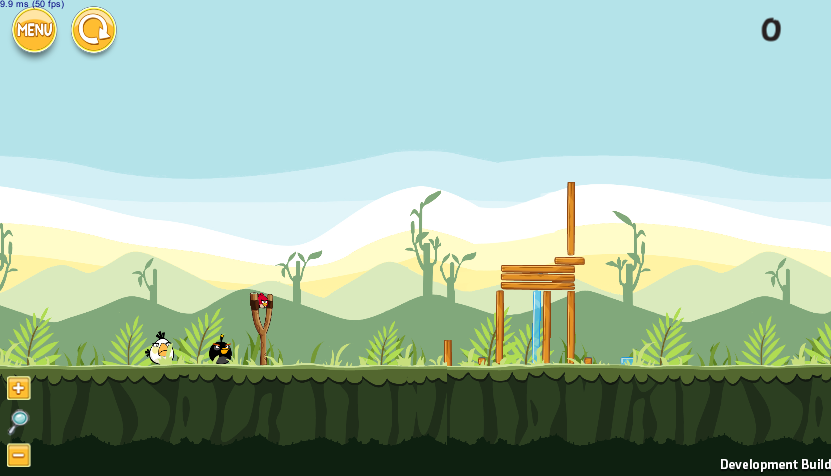
\includegraphics[scale=0.3]{E6.png}
 	\caption{One of the solutions from E6}\label{f:e6}
 \end{figure}


 %Again, you can't simply show a single figure as a result. Maybe show
 %average height, or several best solutions. And always reference the
 %figure - JJ
%************************************************



%%%%%%%%%%%%%%%%%%%%%%%%%%%%%  CONCLUSIONS  %%%%%%%%%%%%%%%%%%%%%%%%%%%%
%
\section{Conclusions and Future Work} 
\label{sec:conclusions}

This paper was developed with
objective of exploring the expressiveness and variability of 
SBPCG with evolutionary techniques
and producing stable structures under gravity.


% Antonio - This is my Proposal for this paragraph
For this aim we have implemented an Evolutionary Algorithm able to optimize 
level structures to meet this criteria. %, like the stability of the 
%constructions.
%Perhaps the level of achievement of the first objective, exploring the 
%expressiveness and variability of 
%SBPCG with evolutionary techniques,
%is not as easily measurable as the other two. It could seem like
%this objective has not been fully accomplished: only one SBPCG method
%has been implemented and tested. However, it was not in the scope of
%this work to test SBPCG in general, but in this particular case, for
%this particular game.
%Considering this, 
The method studied was
sufficiently general and flexible to draw some conclusions about the
topic. SBPCG methods are a potential good solution to offline content
generation but it requires a great amount of problem-specific
knowledge. 
%Like any other form of creative work, 
%The biggest issue may
%be how to measure how good, creative or enjoyable is the piece. 
The more rules the author adds, results tend to be 
%expressiveness starts to get lost as the results are 
variations of the same idea. However, %it is crystal clear
%from the experiments run in this paper that 
a lack of knowledge
will lead to unexpected outcomes.
In our case, the fitness function used the 
stability of the structure and only considered other features %--- overlapping 
%blocks and distance to the ground--- 
to ensure the levels would be valid.
%In experiment \ref{E5} and \ref{E6} height was also taken into account.

 % I am lost in this paragraph. It should be more
 % related to the actual experiments made - JJ

%The second objective, adapting the game to extract data from execution, was 
%certainly achieved. It was also a basic requirement to proceed with the rest of 
%them. The game does provide the data, as long as the input is correctly 
%structured. 
% Although the original intention was to make it available on Linux, 
% currently it can only be executed with the desired behaviour on Windows. 
% Antonio - I think this is not relevant
% Another issue is that the simulation is not easily adaptable. If the fitness 
% function of the EA is changed and needs data that is not included in the 
%output 
% right now, the game would have to be changed and compiled again. 
% Antonio - I would suggest this text instead
%In order to conduct our experiments the Angry Birds simulator (Science Birds) 
%has been adapted to our necessities, yielding now some  other information 
%required to evaluate the individuals of the implemented EA. As this was a 
%bottleneck, experiments \ref{E5} and \ref{E6} used only a physic simulation,
%leaving behind the actual game.
%It would be interesting to obtain other kind of data from both simulations,
%such as the height of the structure and, eventually, its resistance to
%bombardment by angry birds. However, this is left as future work.
The main issue is how we define levels and how the definition %of level 
plays
with the paths of evolution.
Producing stable structures under gravity was %the third objective and
%the closest to the ultimate one. That objective was 
effectively
achieved, but the consequence of evolving in a path of minimum movement 
%or maximum stability
results in squat
structures that are %neither aesthetically pleasing nor 
not playable,
although undeniably sturdy and stable. % and do not have more than a few floors, which could not be very 
%exciting for the players. 
% Antonio - I would add:
% , which could not be very exciting for the players. 
% Tell me what you think of this.
% Floors is not precise. ..more than a few stacked blocks? - Mario 
%The main issue is, then, how we evaluate the levels. In fact this is 
%a matter of how we define what an Angry Birds' level \textit{is} and if that 
%definition matches the fitness function.
%A lot of elements were correct, but the definition was not complete.
 % is also a problem.
%Since we define as
%level as a structure that
%If the key feature in the definition is \textit{stable}, evolution 
%will maximize stability,
%finding %, as in the beginnings of architectural practice,

%We have been successful in,
%evolving free form structures, to find these type. But once we get
%there, we need to go into a different evolution mode that takes into
%account several features as 
Next step would be treating this as a multiobjective optimization problem:
stability is the first, but we can sacrifice a bit of stability for
height or some other aesthetic quality.

% This idea brings us to the last objective, that was not achieved. Without 
% results that match the definition of an Angry Birds level, placing the 
% remaining objects would not have made the level playable. The partial 
% achievement of the third goal, blocked the fourth one as this objective was 
% dependent on the third one.

To conclude on an optimistic tone, this work provides an interesting insight 
into the SBPCG, through the completion---and failure---of the goals we
set out to achieve at the beginning.
%
%In order to improve the results of the method, different constraints could be 
%expressed as multiple objectives. Overlapping blocks and velocity could 
%be treated as minimization objectives and height as a maximization one. % but 
%of course we don't need
                                % to minimize height any more... - JJ
                                % Corrected - Laura

%If we pay attention at the stages of evolution in this work, there is also 
%room for improvement in the genetic operators. For example, the initialization 
%produces a small amount of valid individuals which suggested that an elitist 
%strategy for selection would work best. However, new experiments will help to 
%better balance exploration and exploitation. An interesting addition
%would be to add {\em building} operators that pile blocks on
%structures that are already stable. % Check out this idea, Laura - JJ
 % I like it, let's keep it - Laura

% First a discussion to say if the goal can be achieved using these
% methods. That is, finding stable structures is just a matter of
% adding more to the minimum numbre of blocks or more generations? - JJ

% ---- If we need 5 hours for every run, this is not realistic --- 
% Once we had a generator that meets our expectations, performance could be 
% enhanced by the analysis of the best set of initial parameters using Analysis 
% of Variance (or ANOVA), as presented in \cite{estevez2017statistical}. 

% ---- Some kind of "building" could be combined as genetic operator,
% but that would create structures that are too similar -- JJ
% -------------
% Some options were discarded for time limitations, so these could be main 
%areas 
% of development. The chromosome representation using generative grammatical 
% encoding\cite{hornby2001advantages}, although it would radically change the 
% structure of the method, might ensure that generated levels are consistent. 
% This would require carefully selection the operators that would be the 
%building 
% blocks of the generative grammar.


%Another important issue that needs to be addressed is the time performance. 
%Right now the simulation is the main bottleneck in the execution. One way to 
%speed up the process can be \textit{cleaning} up the current simulation, 
%getting 
%rid of any unnecessary assets while maintaining the bare minimum to
%perform evaluation. 
% However, this will not solve the problem, since the content generator will 
%still need to launch an external executable.
% Antonio - I would not mention future problems

%The communication between the simulation and the content generator is through 
%read and write operations on disk, instead of memory. This could be avoided if 
%both tools were integrated in one.
%If we aim for an online automatic generator, the generator should be 
%integrated in the game and therefore the current execution times would
%be unacceptable. However, if our goal is to 
%generate levels for mixed authorship, as an assistance to developers, it may be 
%a better idea to integrate the simulation in the generator.
% This could be done 
% by approximating in-game physics with real physics, as described in 
% \cite{blum1970stability}. % Expand on this - JJ
% Or maybe eliminate if there's no space - JJ



%----------------------- ACKNOWLEDGEMENTS -----------------------
\begin{acks}
 This paper has been supported in part by DeepBio (TIN2017-85727-C4-2-P).
\end{acks}

\bibliographystyle{ACM-Reference-Format}
\bibliography{angrybirds} 

\end{document}